\documentclass[submission, copyright,creativecommons,sharealike,noncommercial]{eptcs}
\providecommand{\event}{Swarm group}

\newcommand{\yourpath}{Preambles/}
\usepackage{import}
\usepackage{eufrak}
\subimport{\yourpath/}{packages}
\subimport{\yourpath/}{macros}
\subimport{\yourpath/}{tikzstyles}

\subimport{Preambles/}{LocalDefinitions}

\newcommand{\candidates}{\ensuremath{\mathcal{C}} \xspace} 
\newcommand{\range}{\ensuremath{\mathfrak{R}}\xspace}

\title{Liquid Democracy Voting System for the Swarm Platform}
\author{Fabrizio Romano Genovese
	\institute{Swarm Team}
	\institute{Quantum Group \\ University of Oxford}
	\email{fabrizio@swarm.fund}
\and
Jelle Herold
	\institute{Swarm Team}
	\email{jelle@swarm.fund}
}
\def\titlerunning{Liquid Democracy -- Concrete proposal}
\def\authorrunning{F.R.Genovese \& J. Herold}
\usepackage{wrapfig}

\begin{document}

%	\bibliographystyle{eptcs}
	
	\maketitle

	\begin{abstract}
		Here we highlight how the voting system is going to work. We will start briefly reviewing existent solutions, we will proceed sketching the general idea for the voting system on the Swarm Platform and, finally, we will dive into details producing a working algorithm.
	\end{abstract}

\section{Pre-existent solutions}\label{sec:Pre-existent solutions}
	The need to define a voting system is not a new problem for the blockchain community. For instance, if some altcoin is going to hard fork, the developing team will often ask the user base to express a preference about which branch to adopt. It is obvious, then, that in a situation like this some kind of procedure has to be devised to allow people to express this preference, that is, to allow people to vote.
	
	One of the most common ways to deal with this problem is by issuing some voting tokens and creating two addresses that stand for \emph{yes} and \emph{no}. Every user receives a number of tokens equal to the number of coins owned and sends them to one of these two addresses, expressing a preference.
	
	Albeit very simple to implement, this method has many fundamental flaws that make it not suitable for a system that has democracy -- and hence voting -- at its center:
	\begin{enumerate}
		
		\item First of all, a voting procedure like the one highlighted above is very similar to majority voting and, as such, it is cursed by many downsides. One of the biggest achievement of social choice theory is proving that many of the voting systems that people intuitively consider ``fair'' are not fair at all, meaning that they are prone to any sort of manipulation [] or can even be dictatorial []. Voting with tokens as stated above is no exception. 
		
		\item In the very same moment someone votes, the tokens are transferred to the address expressing a preference, and can be publicly seen. This means that a sufficiently skilled user is able to see in real time who is winning the vote. This exposes the system because gives away data that can be employed for any kind of manipulation.
		
		\item ``Real'' tokens can be exchanged while the voting ones remain in one's wallet. This means that voting power is not really related to the quantity of money one owns: In a transaction happening after the voting tokens are issued, the person receiving the real tokens has no voting power whatsoever while, on the other hand, the other person retains the voting power without having real stake.
		
		For instance, someone with a lot of real tokens could sell them all, and then use the voting tokens he retained to vote for a very bad decision for the platform. At this point the tokens he just sold will be depreciated because of this bad decision and the person will be able to buy them back at a fraction of the price, making a profit. 
		
		This means that a very powerful user on the platform could exploit the democratic infrastructure to make direct profits.
		
		\item There is no reputation system. This means that a user voting power is only proportional to the amount of coins owned. A lot of important parameters (how active that user is on the platform, how much money one moves every month, how much that user helped with proposals, \dots) are completely disregarded.
		
		\item Vote delegation is messy, or even not impossible.
	\end{enumerate}
	For these reasons we deemed necessary to steer away from all the pre-existing solutions and design an ad-hoc voting environment that is reasonably fair (according to social choice theory) and suitable to be used on a daily basis.

\section{Range Voting}

	\begin{wrapfigure}{r}{0.5\textwidth}
		\vspace{-10pt}
		\begin{center}
			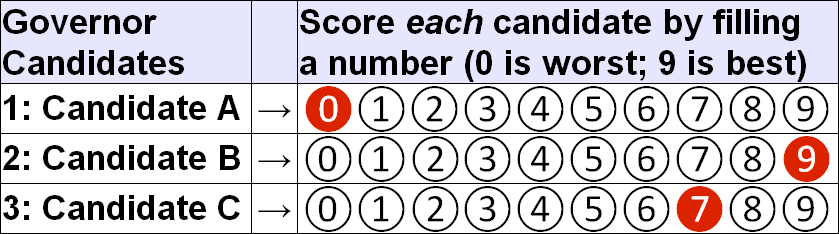
\includegraphics[width=0.48\textwidth]{Voting_Ballot.png}
		\end{center}
		\vspace{-15pt}
		\caption{Range voting ballot [source: Wikipedia]}
		\vspace{-5pt}
	\end{wrapfigure}

	The voting method we choose for the platform is \emph{range voting}. Range voting is one of the fairest voting systems available. In particular, being it a \emph{cardinal} and not an \emph{ordinal}\footnote{These are technical terms of voting theory. You can safely ignore them if you don't know what they mean.} voting system, many of the mathematical results about unfairness and dictatorship, such as [], do not apply.
	
	In range voting, each voter can rank each choice giving a score, for instance from $0$ to $10$, where $0$ stands for ``I absolutely don't like this choice'' and $10$ stands for ``I absolutely love it'' (see for instance Figure~[]). When the voting closes, the scores for each choice are summed, and the choice with more points is the one that wins.
	
	There are many groups that actively advocate for range voting to be adopted in electoral laws all around the world, and in addition to this range voting is also considerd one of the best voting procedure available in company administration (see, for instance [][]). 
	
	To conclude, in choosing the right voting procedure for the Swarm platform we consulted decades of research and study on voting systems to find the best alternative available, and we are fairly convinced that range voting is the one.
	
	\subsection{Reputation}
	Taking into account ``modifiers of the voting power'' is also very easy when one adopts range voting. Let's suppose, for instance, that we want to have a system where the power of a voter is proportional to the number of coins he owns. If voter $A$ owns $n$ coins, then it will be sufficient to multiply by $n$ all the scores that $A$ gives to each candidate. So, for instance, if $A$ owns $10$ coins and ranks a candidate with a score of $5$, that candidate will receive $10*5=50$ points.
	
	To be precise, we want to take into account more parameters than just the quantity of money a voter has to determine the voting power, but now we do not need any new concept to do this. For each user $A$, we will just calculate a multiplier, denoted with $\rho_A$ and called \emph{reputation of $A$}, considering all the parameters that we deem relevant. Again, everything we will need to do to make $A$'s votes proportional to his reputation is to multiply all the scores that $A$ assigns by $\rho_A$.

	\subsection{Drafts}
	Clearly, it may happen that a vote leads to a draft. In range voting this means that there are two or more candidates at the top of the points list having the same score. For instance, imagine we have to elect three people for a company board and there are ten candidates, with their ranking in terms of points as follows:
	\begin{center}
	\begin{tabular}{| l | r |}
		\hline
		\textbf{Candidate} & \textbf{Points}\\
		\hline			
		Candidate 7 & 247\\
		Candidate 2 & 133\\
		Candidate 5 & 102\\
		Candidate 8 & 102\\
		Candidate 10 & 84\\
		Candidate 1 & 58\\
		Candidate 6 & 37\\
		Candidate 3 & 29\\
		Candidate 9 & 14\\
		Candidate 4 & 3\\
		\hline  
	\end{tabular}
	\end{center}
	Since we are selecting only three members for the board, we have to pick the three best performing candidates. This obviously includes candidates $7$ and $2$, but then we are stucked because candidate $5$ and $8$ have the same amount of points. So who who among the two do we choose?
	
	In classic range voting, at this point, another voting round is held. We discussed at length about implementing such a system for Swarm, and we decided that it wasn't a good idea, first because it puts much more stress and responsibility on users that will have to vote two times, and second because it would make the actual code much more complicated and difficult to audit. So we went for a system in which no second round is needed, as follows:
	\begin{itemize}
		\item If there is an ex-aequo situation, we will prefer the candidate with the highest reputation.
		\item If this doesn't solve the problem (there are multiple winning candidates with the same reputation), then the choice is pseudorandom.
	\end{itemize}

\section{The voting algorithm -- Intuitive explanation}

\subsubsection{Desiderata}
	Now that we know what we want, we have to implement it. There are some fundamental desiderata we require:
	\begin{itemize}
		\item The voting should be transparent. This means that all the relevant information should be stored on the blockchain, and every user should be able to calculate the vote outcome independently, as well as to check that is preference was correctly submitted.
		
		\item The voting should be encrypted. As we said in Section~\ref{sec:Pre-existent solutions}, one problem of voting on the blockchain is that people can know who is winning before the voting window closes. To avoid such a situation, every vote should be encrypted and readable only when the voting window closes.
		
		\item Being an active member of the Swarm democracy should increase a member reputation. Swarm values participation, and it makes sense that ``the more you vote, the more your vote becomes powerful''. This is also a way to value the experience and time spent on the platform.
		
		\item The reputation should also be proportional to the amount of Swarm tokens owned. More specifically, if one owns zero Swarm tokens then his voting power should be zero (meaning that has no influence whatsoever).
		
		\item Delegation must be possible. The word ``delegation'' is actually the reason why we talk about \emph{liquid democracy} and not just about \emph{deocracy}. The idea here is that any Swarm member can delegate some other member to vote in his place. This is particularly useful when someone is asked to take a decision, but does not feel to have enough experience or understanding to vote. Instead of wasting his preference, in such situation a user can delegate someone else to vote in his place.
		Imagine, for instance, that Bob is a Swarm user. Bob has to vote to elect members of the administration Board. He reads all the proposals and what every member wants to do, but it is all incredibly technical and out of his skill set. Bob, on the other hand, knows that Alice, a professional trader which he trusts, is on Swarm too. What Bob can do is delegating Alice to vote for him, so that his preference will not be wasted.		
	\end{itemize}

\subsubsection{User experience}
	From the point of view of a Swarm user, voting should be simple. The idea is that you just visit a webpage, and use the ethereum address you have your tokens on as a login. At this point, you are able to see your reputation and all the open voting windows. To vote, it is sufficient to rank each candidate on the webpage and sign your preference with your private key. At this point, the preference is submitted. To improve easy of use, we are working to make such webpage compatible with Nano Ledger S and Trezor, so that signing your petition will just require a couple of clicks.
	
	When the voting window closes and the outcome is calculated, the user should will be able to see it on the very same web page.
	
\subsection{The Voting Algorithm}	










\section{The Algorithm, detailed explanation}
	This section is technical and requires some basic familiarity with mathematics and coding. 

	\begin{definition}
		A \emph{string} $s$ is a finite sequence of characters or digits $s_1 s_2 \cdots s_n$. If $s$ is a string, we will denote with $s[n]$ the \emph{n-th} character of $s$, and with $|s|$ the \emph{length} of $s$. We will abuse this notation and we will often use \emph{strings of strings}, that is, some string $s$ such that $s[n]$, for some $n$, is a string too. In this case, we will denote with $s[n][m]$ the $m$-th entry of the $n$-th entry of $s$.
	\end{definition}	
	
	\begin{definition}
		We will denote with \candidates the \emph{ordered} set of candidates or choices that can be voted for in a given vote. We will denote with \range the set of possible scores a user can assign to each candidate. For instance, if we have three possible choices $A,B,C$ and the range of possible scores goes from $-3$ to $3$, then $\candidates := \{A, B, C\}$ and $\range := \{-3,-2,-1,0,1,2,3\}$. We will moreover denote with $| \candidates|$ and $|\range|$ the number of elements that these two sets have. In our example, $|\candidates | = 3$ and $|\range|=7$.
	\end{definition}
	
	\begin{definition}\label{voting string}		
		We can express the voting of a user as a string $(a,b,c, \dots)$, where $a,b,c \in \range$. $a$ represents the rating given to candidate $A$, $b$ the rating given to candidate $B$ and $c$ the rating given to candidate $C$ and so on. This string is called \emph{voting string}, and its length is clearly equal to $|\candidates|$.
	\end{definition}
	\begin{definition}
 		We denote an user $A$ delegating his/her vote to a user $B$ with $A \to B$.
	\end{definition}
	
	\subsection{The algorythm}
		Here we draft an algorythm to take care of voting. An analysis of this algorythm will be given in the next section.
		\subsubsection{Phase 1: Submitting candidatures}
		
		\begin{itemize}
			\item A contract called $\textbf{CANDIDATES}$ is created. This contract determines from when to when voting is open and is fundamentally a list of strings representing the candidates;
			
			\item An user that wants to run for the election writes a bio and a covering letter and he signs this with his/eth ethwallet private key.
			
			\item The user adds to a public contract a line like this:
			\[
			(\text{ethwallet} \mid \text{hash of the bio} \mid \text{hash of the covering letter})
			\]
			
			\item When the window closes, every new submission is rejected. 
		\end{itemize}
		
		\subsubsection{Guardians and private keys}
			\begin{itemize}
				\item A public key is created out of two secret keys, that will be kept by two different trusted parties (us and the tokensale guys, for instance);
				
				\item The public key is denoted with $pub$, while the secret keys are denoted with $sec_1$ and $sec_2$, respectively. It makes sense to give one of these secret keys to the Estonian non-profit organization that oversees Swarm, if possible.
				
			\end{itemize}
		\subsubsection{Voting window}
			\begin{itemize}
				\item Every person owning an eth wallet (even with no swarm tokens in it) can submit a vote. Every user can see who are the candidates running on our dedicated website. The website just displays the addresses of all the candidates along with their bios and covering letters, ordered by their stake. The fact that $\textbf{CANDIDATES}$ contains this information ensures that we are not providing incorrect/manipulated information about the candidates.
				
				\item An eth contract, called $\textbf{VOTE}$, is created on the blockchain. This contract determines from when to when voting is open and is fundamentally a list of strings representing the users votes.
				
				\item The user vote is a string defined as follows: 
				\[
				(\text{user wallet address}, \text{voting string}, \text{delegation address})
				\]
				Where:
				\begin{description}
					\item[user wallet address] is the eth address of the voter;
					\item[voting string] is a string defined as in Definition~\ref{voting string}, where $\mathfrak{M}$ is the set of all the addresses in \textbf{CANDIDATES}. To be specific, the first entry of the voting string refers to the first candidate in $\textbf{CANDIDATES}$, the second to the second candidate in \textbf{CANDIDATES} and so on.
					
					\item[delegation address] is an eth address.
					
					\item vote strings and delegation addresses are set to some standard value ($0$ for eth address) and $(0,0, \dots, 0)$ for the vote string) if the user does not specify any value.
				\end{description}
			
				\item The user encrypts this string using $pub$ and adds the line to $\textbf{VOTE}$.
			\end{itemize}
		
		\subsubsection{Outcome}
			\begin{itemize}
				\item When the voting window closes, the outcome of the vote is calculated. The secret keys $sec_1$ and $sec_2$ are made public and added to $\textbf{VOTE}$. With this information, any user can decrypt the content of $\textbf{VOTE}$.
				
				\item The outcome is calculated as follows: First, we decrypt $\textbf{VOTE}$ and we copy its content to $\textbf{VOTE'}$. $\textbf{VOTE'}$ is basically a huge database with all the addresses of people who voted, their voting preference and the delegation address specified. 
				
				\item We check that no one used the Swarm foundation address to vote. Since the foundation owns like 33\% of the total swarm tokens, this would be very unfair: Partners can of course vote with their personal wallets but not with the foundation one. Hardcoding this guarantees transparency both for the partners and for the investors.
				
				We scroll $\textbf{VOTE'}$ and check the first address of each string. If a string starting with the Swarm foundation eth address is found, we erase it. We keep doing this until we reach the bottom of the contract. 
				
				\item After this, we have to check that people did not vote two times. This is easy: We scroll the $\textbf{VOTE'}$ database again and check the first address of each string (voter's address). If two or more strings have the same voting address, only the most recent is kept. Since strings are added as votes come, we just have to erase all but the bottommost one.
			
				\item Then we check that all the delegations are correct. This means we have to rule out cases in which there are delegation loops, i.e. we have to deal with situations like $A \to B \to C \to A$ where we have a loop and it is not clear who is voting on behalf of who. To do this we apply the following algorithm:
				
				\begin{itemize}
					\item Call $a,b,\dots$ the entries in $\textbf{VOTE'}$. Starting from $a$, we form a string called \emph{check} as follows:
					\begin{itemize}
						\item The first entry of \emph{check} is $a[1]$ (user wallet address).
				
						\item The next entry of \emph{check} is $a[3]$ (the delegation address).
				
						\item If $a[3]=0$ then the algorithm terminates and we run it on the next entry in $\textbf{VOTE'}$. Otherwise we scroll down \textbf{VOTE'} until we find an entry $n$ such that $n[1] = a[3]$ (we check if the delegated address has voted). If this string does not exists, we then modify \textbf{VOTE'} setting $a[3] = 0$ (delegation is not valid). If it exists, we add $n[1]$ to \emph{check}.
						
						\item We re-run the same procedure starting from $n[1]$.
						
						\item At every step, we check if \emph{check} has repeated entries. Two things can happen:
						
						\begin{itemize}
							\item If we find that repeated entries, then \emph{check} will look like $(a,b,x,c,d, \dots, f, x)$. In this case we modify \textbf{VOTE'} setting $x[3] = c[3] = \dots = f[3] = 0$ (we eliminate the loop setting all the delegations in the loop as not valid); 
							then we start again using the string immediately following $a$.
							
							\item If we don't find repeated entries, we eventually reach the end of \textbf{VOTE'}. In this case we start again using the string immediately following $a$.
						\end{itemize} 
					\end{itemize}
				
				\item At the end of this process, \textbf{VOTE'} will be free of delegation loops. At this point we calculate the outcome as follows:
					\begin{itemize}
						\item For every string $n$ we check that $n[2]$ is a valid voting string, meaning that all the points assigned are in the correct range and the number of entries in the string equals the number of candidates. Mathematically, this means that every entry in $n[2]$ is in $\mathfrak{M}$ and that the lenght of $n$ is $|\mathcal{N}|$. If this is not the case we set $n[2]$ to the string made of $|\mathcal{N}|$ entries in which every entry is $0$. We will denote this string just with $\mathbf{0}$.
					
						\item For every string $n$, call $\sigma_{n[1]}$ the stake of $n[1]$. If $n[3] = 0$ (no delegation), then $n[2] = \sigma_{n[1]} n[2]$, meaning that we multiply every entry of $n[2]$ by $\sigma_{n[1]}$. If $n[3] = a$, then $n[2] = \mathbf{0}$ and $\sigma_{k[1]} = \sigma_{n[1]} + \sigma_{k[1]}$ (we transfer the stake to the delegated user), where $k$ is the entry such that $k[1] = a$ (having eliminated loops there is only one such string $k$).
						
						
						\item We calculate the string \emph{outcome} as $\sum_{n \in \textbf{VOTE}} n[2]$ (we are summing all the points in all the voting strings componentwise).
						
						\item The elected candidates are the ones with the highest amount of points in \emph{outcome}. For instance, if $\emph{outcome} = (234, 152, 36)$ then the candidate corresponding to the first string entry is the winner.
						
						\item We have to elect three candidates for the board. We proceed as follows: We consider the three candidates having the biggest amount of points. If these are more than three, we further order them considering their stake, meaning that if $A,B$ have the same amount of points but the stake of $A$ is bigger than the stake of $B$, then $A$ is preferred. If we still have more than three candidates ex-aequo, then we randomly chose three.
					\end{itemize}
				\end{itemize}
			\end{itemize}

\section{The code}
	The source code of the algorithm, when completed, will be appended to this section. It will only contain the core functions dealing with smart contracts. If you want a more detailed coverage, comprising the front end part too, please refer to our github repo [].


	\subsection{Analysis}
		With this algorithm we solve a shitload or problems. No one is able to see who voted for who and what is the delegation structure until the vote ends. The fact that the public key is obtained from two different secret keys means that not even the guardians are able to do this alone. The guardians should agree to fuck the platform sharing their secret keys and accessing the votes outcome while the voting window is still open. This is obviously possible and this is why the guardians should be two trusted and independent entities.
		
		Users are able to delegate their vote to someone. If this delegation doesn't work well (loops, the delegate didn't vote) then the system falls back on the user preference. This means that if your delegate is a dickhead your vote is not wasted.
		
		Since the stake is taken to be the one at the closing of the voting window, people cannot really fiddle with their token in the hope to increase their voting stake. Moreover, the voting is not made sending tokens to this or that address, and no tokens are locked in the process, so everyone can move his/her tokens as he/she pleases during a voting. The only thing to keep in mind is that your stake will be the one at the end of the closing window.
		
		
\end{document}


